\documentclass{article} % For LaTeX2e
\usepackage{iclr2026_conference,times}

% Optional math commands from https://github.com/goodfeli/dlbook_notation.
\input{math_commands.tex}

\usepackage{hyperref}
\usepackage{url}
\usepackage{graphicx}
\usepackage{booktabs}
\usepackage{multirow}

% \iclrfinalcopy % Uncomment for camera-ready

\title{Structure and Dynamics of Agentic Innovation}

\author{Anonymous authors\\
Paper under double-blind review}

\newcommand{\fix}{\marginpar{FIX}}
\newcommand{\new}{\marginpar{NEW}}

\begin{document}

\maketitle

\begin{abstract}
We study scientific innovation as a dynamical system: the \emph{state} is a
citation network of research ideas distilled from published papers, and the
\emph{dynamics} are LLM agents that navigate the network and write new ideas
(and links) back into it. Agents propose ideas freely; each proposal is
scored by whether a similar paper published \emph{after} the agent model's
training cutoff realizes it, verified by literature search and graded by an
LLM judge on a six-level scale across three venue-recognition tiers
(headline accuracy: share of ideas matched at level $\geq 2$, ``same
specific problem''). On a
16{,}208-node network built from NeurIPS, ICLR, ICML, and AAAI papers
(2020--2024), we manipulate a single \emph{specialization dial}: the number
of corpus papers an agent is allowed to read, from 400 up to the whole
corpus. We find (i) an inverted-U in per-idea anticipation accuracy peaking
at a scope of 800 papers---a coherent sub-area, not one topic---with
unrestricted generalists strictly worst on every tier; (ii) idea production
falls monotonically as scope widens; (iii) team size is a pure throughput
knob: per-idea accuracy is flat from 10 to 150 agents while absolute hits
scale linearly, because agents are effectively independent---across 10{,}300
actions we observe a single cross-agent citation of a generated idea.
Strikingly, deleting all 80{,}962 citation edges from the initial network
\emph{helps} generalists (tier-1 accuracy 37\% vs.\ 20\%, with more ideas
produced): agents navigate semantically, not structurally, and the human
citation topology acts as a distractor rather than a scaffold.
Consistently, agent-written links have near-constant semantic reach
regardless of scope, are degree-decoupled (unlike the preferential
attachment that built the corpus), and preferentially target recent
frontier papers. Our results position reading scope---not team size or
citation structure---as the operative lever on the quality of
machine-generated research ideas.
\end{abstract}

\section{Introduction}

Can a system of LLM agents, given the recent scientific literature as a
navigable network, anticipate where science is going next? And if so, what
features of the system---the structure of the network, the behavioral
constraints on the agents, the size of the team---determine how well it
does? These questions matter both for the emerging practice of automated
research ideation \citep{lu2024aiscientist,si2024llmideas} and for the
science of science, where the interplay between knowledge structure and
discovery has long been studied on human data
\citep{fortunato2018science,uzzi2013atypical,wu2019teams}.

We formalize the setting as a dynamical system. The \textbf{state} is an
\emph{idea network}: each node is a one-paragraph distillation of a
published paper, and directed edges are citations. The \textbf{dynamics}
are LLM agents that act on the state through a small action set---semantic
search, browsing a node and its neighbors, random jumps, adding or removing
links, and \emph{generating} a new idea node that cites the ideas it builds
on. State and dynamics are inseparable: every generated node and link
becomes part of the network that all agents subsequently navigate
(a stigmergic channel \citep{theraulaz1999stigmergy}).

Evaluation exploits the arrow of time. The corpus contains only papers
published before the agent model's training cutoff (September 2024). A
generated idea scores only if a paper published \emph{after} the cutoff
realizes it---\emph{anticipation}, verified by live literature search
\citep{kinney2023s2,priem2022openalex} and graded by an LLM judge on a
six-level realization scale, reported across three cumulative
venue-recognition tiers (top venues, top+second-tier venues, any published
paper). Matches to pre-cutoff papers or to corpus members are excluded, so
memorization cannot score.

Our central manipulation is deliberately minimal: a single
\emph{specialization dial}. Each ``specialist'' agent draws one topic from
a 50-topic pool and may only \emph{read} (search, browse, jump within, and
hence cite) the $m$ corpus papers nearest its topic anchor in embedding
space, with $m \in \{400, 800, 1600, 3200, 6400\}$; writing is always
unconstrained. Unrestricted generalists provide the $m=\infty$ endpoint. A
second manipulation varies team size $N \in \{10, 50, 100, 150\}$ at fixed
per-agent interaction depth.

\textbf{Findings.}
\begin{itemize}
\item \textbf{An inverted-U in idea quality over reading scope
  (Sec.~\ref{sec:dial}).} Per-idea anticipation accuracy peaks at $m=800$
  (tier-1 acc@$\geq$2 of 41\% vs.\ 20\% for generalists), and every scoped
  condition beats the unrestricted generalists on every tier. Measured
  region purity shows $m=800$ is a coherent \emph{sub-area neighborhood}
  (own-topic share only 5--60\%), suggesting the sweet spot is ``focused
  but not starved'': narrow enough to force depth, wide enough to contain
  recombination material.
\item \textbf{Quantity falls monotonically with scope
  (Sec.~\ref{sec:dial}).} Narrow readers commit to ideas sooner and
  produce more of them (83 at $m=400$ vs.\ 50 for generalists over the
  same 80 rounds); generalists spend their actions wandering and curating.
\item \textbf{Team size is a throughput knob, not a quality knob
  (Sec.~\ref{sec:scaling}).} From $N=10$ to $N=150$ generalists at fixed
  depth, per-idea accuracy is flat (21--28\%) while absolute hits grow
  linearly. The mechanism is stark: agents are effectively independent.
  Across all scaling runs (575 ideas, 10{,}300 actions) not one agent
  cited another agent's generated idea.
\item \textbf{The citation structure is a distractor, not a scaffold
  (Sec.~\ref{sec:noedges}).} Deleting every initial citation edge makes
  generalists \emph{better}: 60 ideas at 37\% tier-1 accuracy vs.\ 50 at
  20\% with edges, under otherwise identical conditions. Deprived of
  neighbors to wander through, agents commit to pure semantic-search
  navigation (first idea at round 8 instead of 17) --- and spontaneously
  rebuild structure, adding 53 links of their own to the edgeless graph.
\item \textbf{The dynamics have a characteristic ``handwriting''
  (Sec.~\ref{sec:structure}).} The semantic reach of agent-written links
  is nearly invariant to scope (median cosine distance 0.144--0.153,
  slightly \emph{below} the 0.179 of real citations): constraints move
  \emph{where} agents write, not \emph{how far} they link. Agent citations
  are degree-decoupled---the median cited paper has in-degree 0--2, versus
  23 for the target of a real citation edge---and strongly
  recency-seeking (51\% of citations target papers from the corpus's final
  two years, vs.\ 8\% for real edges). LLM dynamics grow the network by a
  different law than the preferential attachment
  \citep{barabasi1999emergence} that grew it.
\end{itemize}

Together these results suggest that in the current regime, the quality of
machine-generated research ideas is governed by how each agent's reading is
situated in the knowledge structure, while multi-agent organization
contributes parallelism but not yet collaboration. We release our full
event logs, evaluation verdicts, and code. % TODO: release URL

\section{Related work}

\textbf{LLM research ideation.} Recent systems generate research ideas or
entire papers with LLMs \citep{lu2024aiscientist}, and human studies find
LLM-generated ideas can be judged more novel than expert ideas
\citep{si2024llmideas}. Evaluation in this literature relies mostly on
human or LLM preference judgments of the ideas themselves. We instead
score \emph{anticipation}: an idea counts only if the future literature
realized it, an outcome measure that needs no human panel and cannot be
gamed by fluent writing alone.

\textbf{Science of science.} Large-scale studies of human science link
discovery to network structure: atypical combinations of prior work
predict impact \citep{uzzi2013atypical}, small teams disrupt while large
teams develop \citep{wu2019teams}, and citation networks grow by
preferential attachment \citep{barabasi1999emergence,fortunato2018science}.
We port these questions to a controlled substrate where the ``researchers''
are LLM agents whose information diet can be intervened on directly---an
experiment impossible with human scientists.

\textbf{Multi-agent LLM systems.} Most LLM multi-agent frameworks
coordinate through explicit messaging. Our agents interact only
stigmergically \citep{theraulaz1999stigmergy}, through traces left in a
shared artifact---the mechanism by which real science coordinates through
the literature itself. Our finding that this channel stays essentially
unused at present scales (Sec.~\ref{sec:structure}) quantifies how far
current agent teams are from literature-mediated collaboration.

\section{The environment: state and dynamics}
\label{sec:framework}

\subsection{State: an idea network from four venues}

We collect the 16{,}208 papers published at NeurIPS, ICLR, ICML, and AAAI
between January 2020 and August 2024 with at least 25 citations, via the
Semantic Scholar Open Data Platform \citep{kinney2023s2}. Each paper's
title and abstract are distilled by an LLM into a self-contained
one-paragraph \emph{idea}. Citation edges among corpus members are
recovered from Semantic Scholar (references and citations arms) augmented
with OpenAlex \citep{priem2022openalex}, yielding 80{,}962 edges (6.4\% of
nodes isolated). Ideas are embedded with a sentence encoder
\citep{xiao2023bge}; embeddings define semantic search, agent scopes, and
the 2-D maps below (PCA + t-SNE \citep{vandermaaten2008tsne}).

\subsection{Dynamics: agents and actions}

Agents share one action interface: \texttt{search} (semantic query, top-$k$
over readable nodes), \texttt{browse} (read a node and its in/out
neighbors), \texttt{sample\_frontier} (random jump within readable scope),
\texttt{generate} (add a new idea node with citations to the ideas it
builds on), \texttt{add\_links}/\texttt{remove\_links} (curate existing
edges). Each agent is a single LLM (\texttt{gpt-5}, medium reasoning) with
a rolling memory of its last 20 action--result pairs and no other channel
to teammates. Agents act in round-robin; one \emph{round} = every agent
acts once. There is no generation budget: whether and when to write is the
agent's choice, so idea count is an outcome variable. Generated nodes and
edges immediately join the shared state.

\subsection{The specialization dial}
\label{sec:scopes}

A specialist draws one topic from a pool of 50 corpus-derived subfields
(clustering + LLM naming; seeded draws, distinct within a run). Its
\emph{readable region} is the $m$ corpus papers nearest the topic anchor
in embedding space (an equal-mass region; the radius adapts per topic).
Reading, searching, jumping, \emph{and citing} are confined to this
region---citing means having read---while the content of generated ideas
is unconstrained. We sweep $m \in \{400, 800, 1600, 3200, 6400\}$
(conditions C2--C6); unrestricted generalists are C1 ($m=\infty$). All
conditions use $N{=}10$ agents, 80 rounds, and the same seed, so topic
draws are identical across the sweep and only the radius varies.

Because topics vary in size (natural partition: median 228 papers, range
44--1096), an $m=800$ region is \emph{not} one topic: measured own-topic
purity is 5--60\% (median $\sim$35\%), i.e., a coherent sub-area
neighborhood containing the topic plus its semantic neighbors. This is
why we treat $m$ as a continuous specialization dial rather than a
one-topic/many-topic dichotomy.

\section{Evaluation: search-verified anticipation}
\label{sec:eval}

For each generated idea we extract three literature-search queries
(problem, method, combination), retrieve candidates from Semantic Scholar
and OpenAlex, and have an LLM judge grade each candidate's realization
level on a six-point scale: 0 (different problem) through 3 (same problem,
same method family) to 5 (same problem, mechanism, and key design
choices). Candidates published on or before the training cutoff
(2024-09-30) and candidates whose titles match corpus members are
excluded before scoring, so neither memorization nor retrieval of the
corpus can score. Near-duplicates of corpus ideas (embedding cosine
$\geq 0.95$) are floored to level 0.

Scores are reported in three cumulative recognition tiers:
\textbf{tier~1} counts realizations in 60 top venues (the 58 CCF-A
venues plus COLM and RLC) or papers with $\geq 50$ citations;
\textbf{tier~2} additionally admits CCF-B venues or $\geq 10$ citations;
\textbf{tier~3} admits any published paper. Per tier we report the mean
best realization level and acc@$\geq$2, the share of ideas whose best
match reaches level 2 (same specific problem)---our headline accuracy;
higher thresholds ($\geq$3, $\geq$4, $=$5) are recorded in the released
verdicts.

\section{Experiment 1: the specialization dial}
\label{sec:dial}

\begin{table}[t]
\caption{The specialization dial: $N{=}10$ agents, 80 rounds, one seed.
Read scope $m$ is the number of corpus papers each agent may read;
writes are always free. Each tier cell reports acc@$\geq$2 (share of
ideas realized at level $\geq 2$ by a post-cutoff paper in the tier;
hits in parentheses) and the mean best realization level.}
\label{tab:dial}
\begin{center}\small
\begin{tabular}{lrrccc}
\toprule
 & \textbf{scope $m$} & \textbf{ideas} & \textbf{tier-1 acc (hits) / mean} &
 \textbf{tier-2 acc / mean} & \textbf{tier-3 acc / mean} \\
\midrule
C2 & 400   & \textbf{83} & 36\% (30) / 0.89 & 47\% / 1.19 & \textbf{89\%} / \textbf{2.48} \\
C3 & 800   & 74 & \textbf{41\% (30) / 1.04} & \textbf{53\% / 1.38} & 84\% / 2.43 \\
C4 & 1600  & 67 & 30\% (20) / 0.78 & 39\% / 1.04 & 60\% / 1.60 \\
C5 & 3200  & 55 & 27\% (15) / 0.69  & 40\% / 1.05 & 73\% / 2.02 \\
C6 & 6400  & 54 & 30\% (16) / 0.74  & 41\% / 1.06 & 78\% / 2.22 \\
C1 & $\infty$ & 50 & 20\% (10) / 0.50 & 26\% / 0.64 & 62\% / 1.68 \\
\bottomrule
\end{tabular}
\end{center}
\end{table}

\begin{figure}[t]
\begin{center}
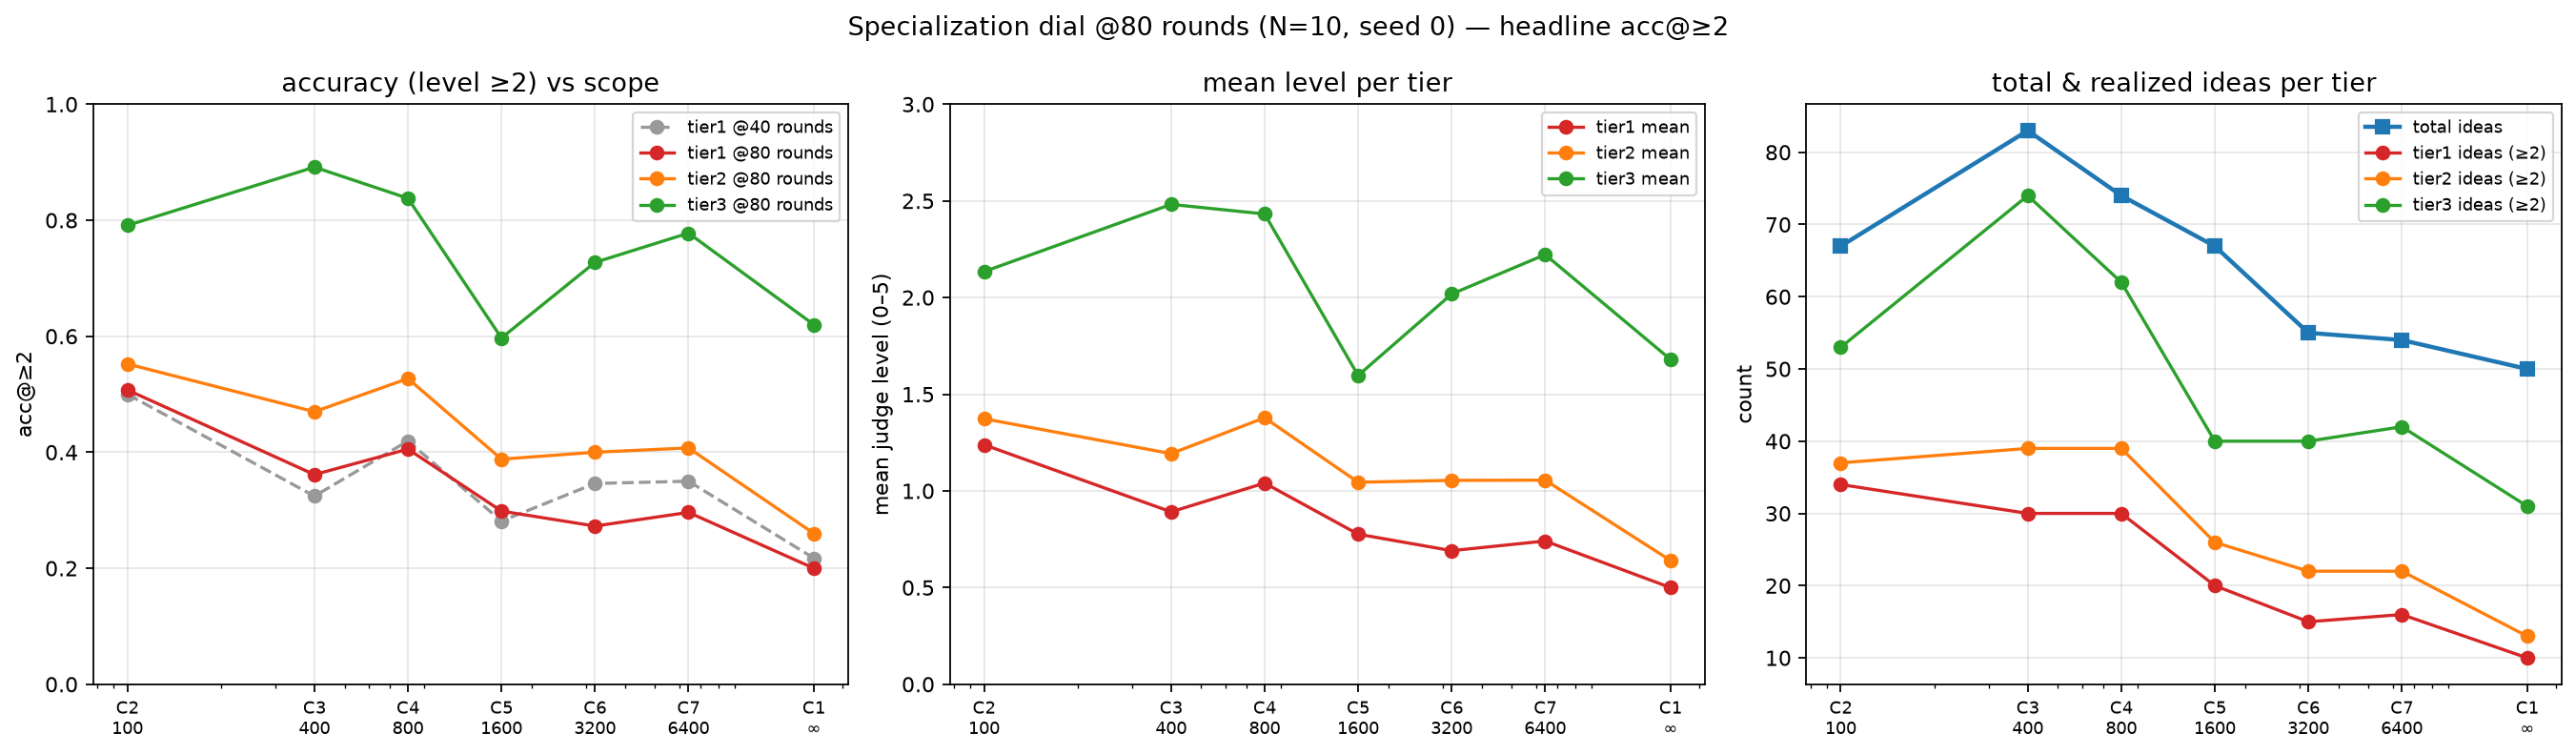
\includegraphics[width=\linewidth]{mass-dial-800-summary.png}
\end{center}
\caption{The specialization dial at 80 rounds. Left: acc@$\geq$2 per tier
vs.\ read scope (log axis); the gray dashed line is the tier-1 curve at
the 40-round midpoint, whose deviations from the 80-round curve
illustrate small-$n$ noise. Middle: mean
realization level. Right: idea production and absolute tier-1 hits.}
\label{fig:dial}
\end{figure}

Table~\ref{tab:dial} and Figure~\ref{fig:dial} give the core result.

\textbf{A mild inverted-U peaking at a sub-area scope.} Tier-1 accuracy
runs 36\% $\to$ \textbf{41\%} $\to$ 30\% $\to$ 27\% $\to$ 30\% $\to$ 20\%
as scope widens; mean realization level tracks the same shape. The
$m{=}800$ condition leads on rate and on tier-1/2 mean level, and ties
$m{=}400$ on absolute tier-1 hits. Both the narrow side (fewer recombination options; topics
with semantically diffuse regions produced agents with zero output) and
the broad side (unfocused wandering) underperform the sub-area
neighborhood.

\textbf{Constraint beats freedom everywhere.} Every scoped condition
dominates the unrestricted generalists on every tier, by rate and by
absolute hits. Moreover the generalists' accuracy \emph{fell} from 22\%
to 20\% when the run was extended from 40 to 80 rounds: the marginal
quality of freely-roaming exploration decays.

\begin{figure}[t]
\begin{center}
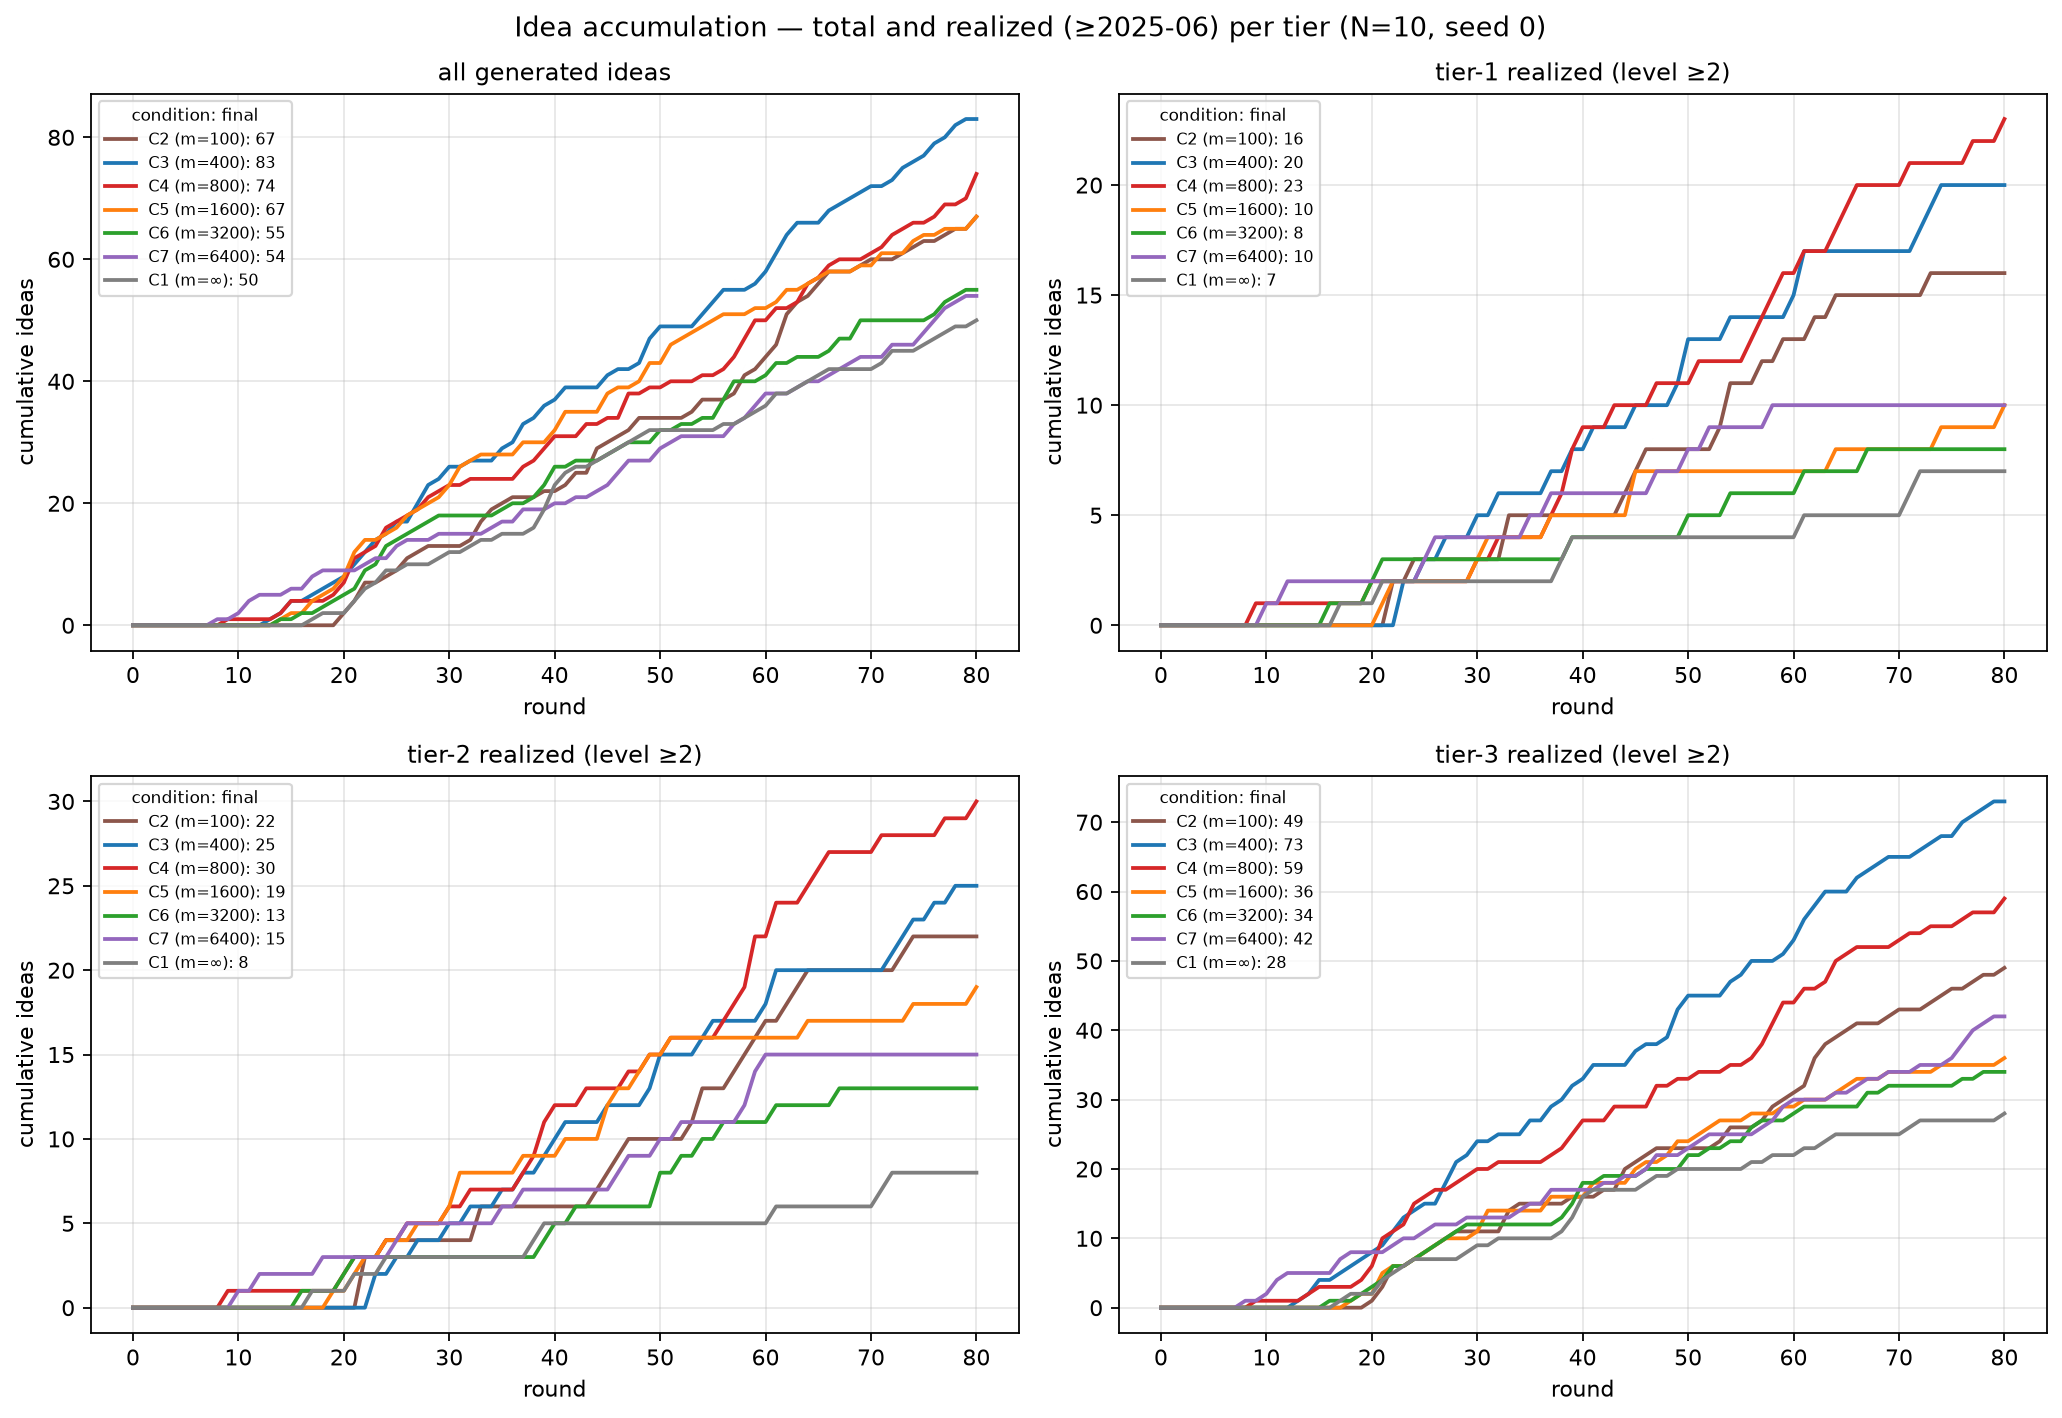
\includegraphics[width=0.72\linewidth]{mass-dial-accumulation.png}
\end{center}
\caption{Cumulative idea production over rounds. All conditions start
producing between rounds 8--17; the production gap is a
\emph{steady-state rate} effect, not a head start: narrow scopes settle
into $\sim$1 idea/round while broad scopes run at $\sim$0.65/round with
recurring plateaus where agents fall back into exploration. No curve
saturates by round 80.}
\label{fig:accum}
\end{figure}

\textbf{Narrow readers ship; broad readers browse.} Idea production is
strictly monotone in scope (83, 74, 67, 55, 54, 50), and
Figure~\ref{fig:accum} shows why: after a comparable exploration onset
(first team idea between rounds 8 and 17; median personal onset round
21--24), narrow scopes settle into a faster and steadier production
rate, while broad scopes stall in recurring exploration plateaus.
Generalists redirect effort into curation: they performed 71
\texttt{add\_links} actions versus 23--38 for scoped conditions.

\textbf{What feeds a realized idea.} The event logs let us trace each
idea's provenance: we take the generating agent's preceding 20 actions
(exactly its FIFO memory window) and classify every read in that window
by the navigation channel that produced it---the node was surfaced by an
earlier \emph{search}, exposed as a neighbor \emph{link} in an earlier
browse, delivered by a random \emph{jump}, or is the agent's \emph{own}
earlier idea. Table~\ref{tab:provenance} aggregates all 1{,}069
evaluated ideas across our experiments. Realized and unrealized ideas
are preceded by the \emph{same volume} of reading ($\sim$10.5 reads);
what differs is its composition. Ideas realized in recognized venues
(tier~1) grew out of windows with more search-driven reads (6.27
vs.\ 5.45), fewer link-driven reads (3.23 vs.\ 3.82), fewer jumps, and
almost no re-reading of the agent's own output. This is the per-idea
mirror of the structural ablation in Sec.~\ref{sec:noedges}: material
found by directed semantic search feeds anticipation; material found by
following citation links does not.

\begin{table}[t]
\caption{Provenance of the reading that precedes each generated idea:
average composition of the generating agent's 20-action lookback window
(= its memory), grouped by realization outcome (tiers are cumulative;
``unrealized'' = no tier-3 match at level $\geq 2$). Pooled over all
1{,}069 evaluated ideas from every run in the paper.}
\label{tab:provenance}
\begin{center}\small
\begin{tabular}{lrcccccc}
\toprule
 & $n$ & \textbf{reads} & \textbf{searches} &
 \textbf{search-fed} & \textbf{link-fed} & \textbf{jump-fed} &
 \textbf{own-idea} \\
\midrule
tier-1 realized & 301 & 10.48 & 6.05 & \textbf{6.27} & \textbf{3.23} & 0.92 & 0.06 \\
tier-2 realized & 404 & 10.46 & 5.97 & 6.15 & 3.31 & 0.95 & 0.05 \\
tier-3 realized & 767 & 10.62 & 5.88 & 6.09 & 3.49 & 0.96 & 0.08 \\
unrealized      & 302 & 10.50 & 5.86 & 5.45 & 3.82 & 1.06 & 0.17 \\
\bottomrule
\end{tabular}
\end{center}
\end{table}

\section{Experiment 2: team size}
\label{sec:scaling}

\begin{table}[t]
\caption{Scaling generalist teams at fixed per-agent depth (30 rounds
each, one seed). The $N{=}10$ point is the 30-round prefix of C1.
Per-idea accuracy is flat; absolute hits scale with output.}
\label{tab:scaling}
\begin{center}\small
\begin{tabular}{rrccc}
\toprule
\textbf{$N$} & \textbf{ideas (per agent)} & \textbf{tier-1 acc (hits) / mean} &
\textbf{tier-2 acc / mean} & \textbf{tier-3 acc / mean} \\
\midrule
10  & 12 (1.2)  & 25\% (3) / 0.67  & 42\% (5) / 1.08  & 75\% (9) / 2.00 \\
50  & 103 (2.1) & 21\% (22) / 0.55 & 34\% (35) / 0.86 & 71\% (73) / 1.98 \\
100 & 180 (1.8) & 24\% (44) / 0.61 & 33\% (60) / 0.83 & 69\% (124) / 1.87 \\
150 & 280 (1.9) & 28\% (77) / 0.66 & 38\% (105) / 0.95 & 68\% (190) / 1.86 \\
\bottomrule
\end{tabular}
\end{center}
\end{table}

\begin{figure}[t]
\begin{center}
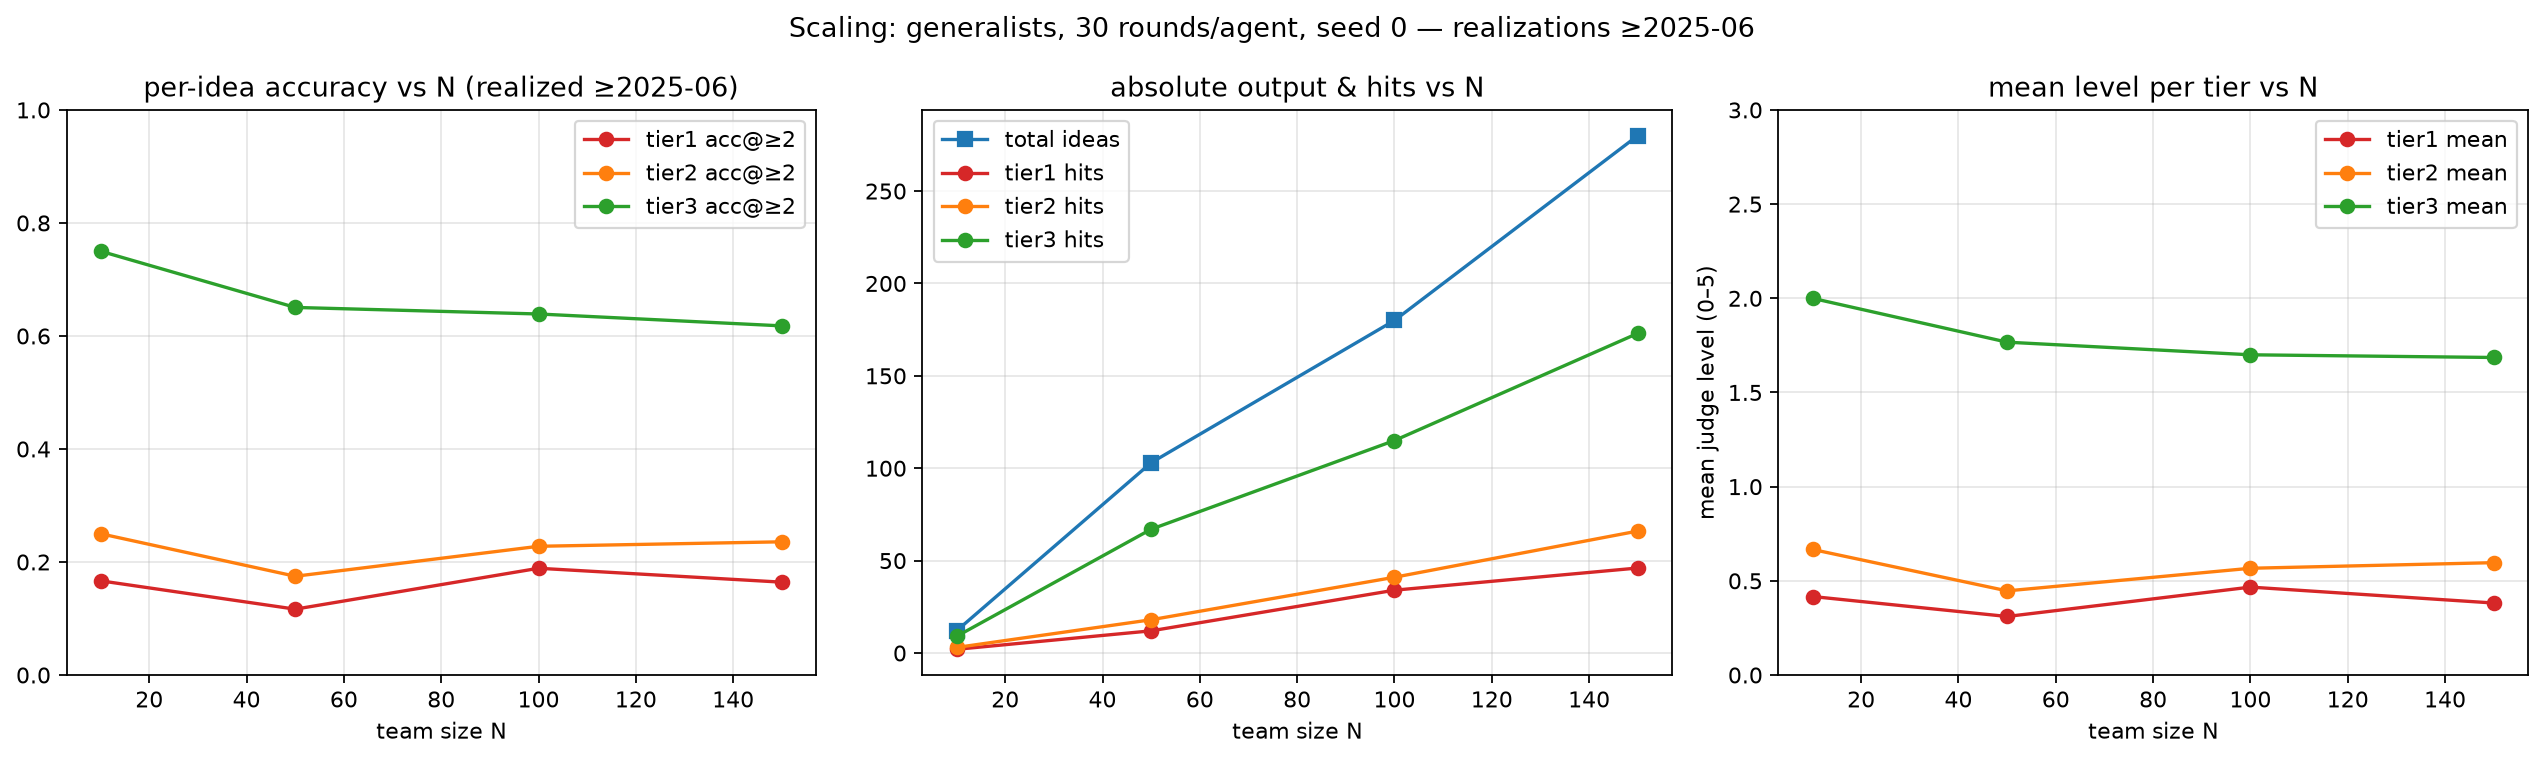
\includegraphics[width=\linewidth]{scaling-summary.png}
\end{center}
\caption{Team-size scaling at fixed per-agent depth. Left: per-idea
accuracy is flat in $N$. Middle: total output and absolute hits grow
linearly. Right: per-capita output is constant; stigmergic coupling (citations of
teammates' generated ideas) is zero throughout (Sec.~\ref{sec:scaling}).}
\label{fig:scaling}
\end{figure}

Holding per-agent depth fixed at 30 rounds and growing the team from 10
to 150 generalists (Table~\ref{tab:scaling}, Figure~\ref{fig:scaling}),
per-idea accuracy stays in the 21--28\% band on tier~1---the $N{=}10$
value rests on 3 hits and is within noise of the rest---while
absolute tier-1 hits grow essentially linearly (3, 22, 44, 77). Team
size buys throughput, not per-idea quality.

The mechanism is that the agents are, in practice, independent samplers.
Across all four scaling runs (575 generated ideas, 10{,}300 actions),
\textbf{zero} citations of another agent's generated idea occurred, and
only two self-citations; in the dial conditions of
Sec.~\ref{sec:dial} (which run 80 rounds), 113 of 114 citations of
generated nodes were \emph{self}-citations---agents building private
research agendas---and exactly one crossed agents. The stigmergic write
channel is active (new nodes join the shared graph), but the read-back
channel is essentially silent: 383 new nodes among 16{,}208 corpus nodes
are simply too rare for semantic search to surface. Making teammates'
contributions discoverable (e.g., recency-weighted search or frontier
sampling) is, on this evidence, the necessary condition for genuine
collaboration effects---and the natural next intervention.

\section{Experiment 3: is the citation structure a scaffold?}
\label{sec:noedges}

\begin{table}[t]
\caption{Exploration-channel ablations: identical to C1 (10 generalists,
80 rounds, same seed and corpus) except the initial network carries no
citation edges (top) or random jumps are disabled (middle). Removing
wandering channels improves output without hurting accuracy; removing
the citation structure improves both.}
\label{tab:noedges}
\begin{center}\small
\begin{tabular}{lrccc}
\toprule
 & \textbf{ideas} & \textbf{tier-1 acc (hits) / mean} &
 \textbf{tier-2 acc / mean} & \textbf{tier-3 acc / mean} \\
\midrule
no edges & 60 & \textbf{37\% (22) / 0.93} & \textbf{43\% / 1.07} & \textbf{75\% / 1.97} \\
no jumps & \textbf{63} & 24\% (15) / 0.62 & 27\% / 0.71 & 73\% / 1.92 \\
C1 (full) & 50 & 20\% (10) / 0.50 & 26\% / 0.64 & 62\% / 1.68 \\
\bottomrule
\end{tabular}
\end{center}
\end{table}

If agents used the citation network as a navigational scaffold, deleting
its edges should hurt. It does the opposite (Table~\ref{tab:noedges}):
with an edgeless initial graph, the same generalist team produces 20\%
more ideas at nearly double the tier-1 accuracy (37\% vs.\ 20\%)---
approaching the dial's $m{=}800$ optimum of 41\%---and starts generating
at team round 8 instead of 17.

The mechanism follows from Sec.~\ref{sec:structure}: agents discover
papers by semantic search, not by traversing references. With edges
present, \texttt{browse} surfaces each node's citation neighborhood, and
agents wander along the \emph{human} citation topology---which pulls
toward older, hub-heavy regions that their own attachment behavior
demonstrably avoids. Removing the edges removes the distractor: browsing
degenerates to reading, navigation collapses onto semantic search, and
exploration converges faster on writeable niches. Notably, the agents do
not leave the graph bare: they spontaneously performed 65 curation
actions, adding 53 links of their own to the edgeless network---they
rebuild structure, but by their own semantic logic rather than the
corpus's citation logic.

A companion ablation disables the other wandering channel: random jumps
(\texttt{sample\_frontier}). The effect points the same way but is much
smaller (Table~\ref{tab:noedges}, middle row: 63 ideas at 24\% vs.\ 50
at 20\%)---unsurprisingly, since C1 agents only jumped $\sim$20 times
in 800 actions. The citation neighborhood, not serendipitous jumping,
is the dominant distractor. We caution that these are single seeded
runs per arm (22/60 and 15/63 vs.\ 10/50 hits); the directions, the
mean-level gaps, and the behavioral signatures are mutually consistent,
but replication is needed before the strongest reading.

\section{Analysis: how the dynamics rewrite the state}
\label{sec:structure}

\begin{figure}[t]
\begin{center}
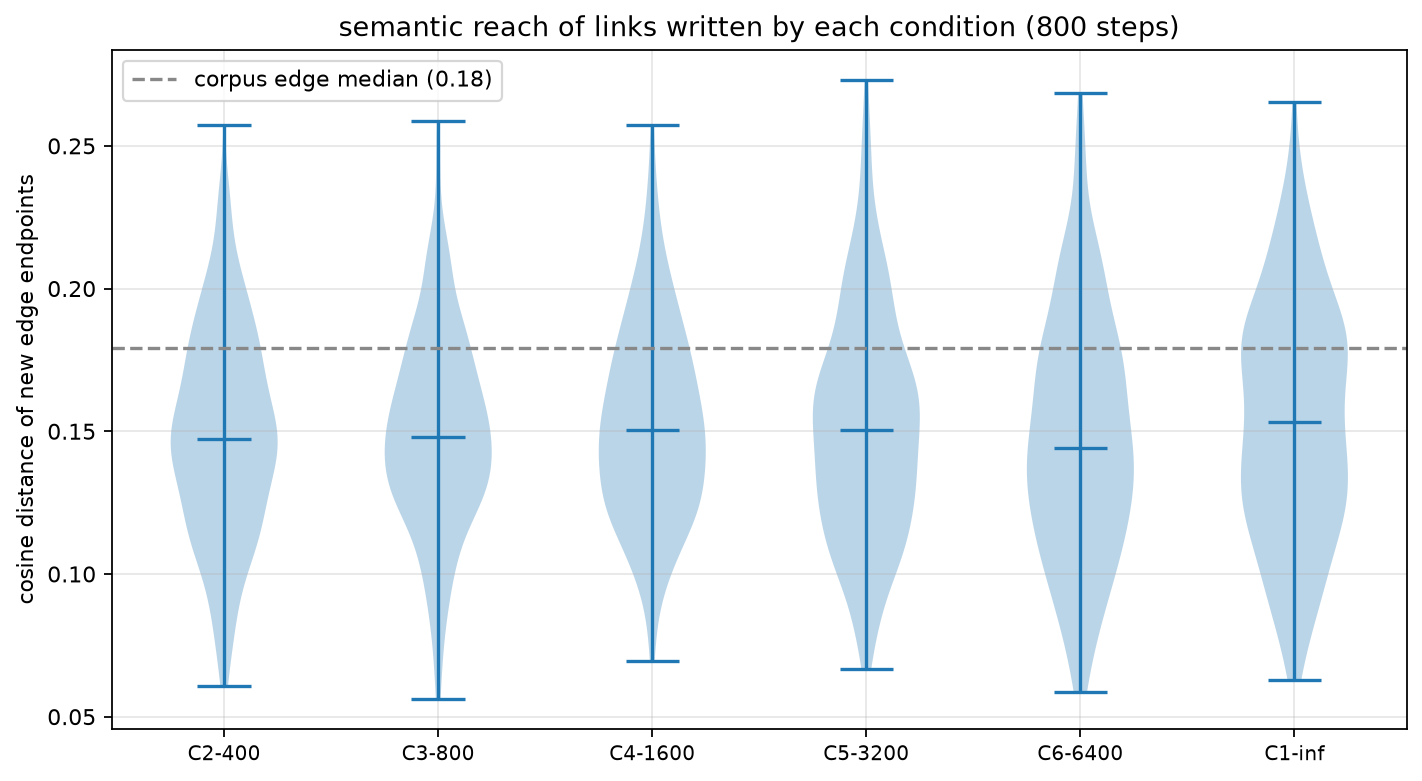
\includegraphics[width=0.7\linewidth]{mass-dial-edge-reach.png}
\end{center}
\caption{Semantic reach of newly written links (cosine distance between
endpoints), per condition. The dynamics' ``handwriting'' is nearly
invariant to the reading constraint, and slightly tighter than real
citation edges (dashed).}
\label{fig:reach}
\end{figure}

We compare the links written by each condition (generate citations plus
curation edges) against the 80{,}962 human citation edges that built the
corpus.

\textbf{Invariant handwriting.} The median semantic distance between the
endpoints of agent-written links is 0.144--0.153 across all six
conditions---a band of width 0.009---versus 0.179 for real citations
(Figure~\ref{fig:reach}). Cross-topic rates hug the corpus baseline
(58--75\% vs.\ 62\%). Reading constraints move \emph{where} an agent
writes, not \emph{how far} its links reach; the local radius of citation
appears to be an intrinsic property of the LLM dynamics.

\textbf{Degree-decoupled, recency-seeking attachment.} Real citation
edges concentrate on hubs: the median target of a corpus edge has
in-degree 23. Agent-written links are nearly degree-blind: median target
in-degree 0--2, against a uniform-selection baseline of 1 (mean 11.6
vs.\ uniform 5.0, i.e., only a mild hub tail). The reason is the
discovery channel: agents find papers by semantic search, which is
degree-agnostic, whereas human discovery historically flows through
reference lists, the visibility cascade that produces preferential
attachment \citep{barabasi1999emergence}. Instead of heat, agents seek
freshness: 51\% of the $m{=}800$ condition's citations target papers
from 2023 onward, versus 8\% of real citation edges. Two growth laws,
one state: the human dynamics that built the network and the LLM
dynamics extending it obey different attachment rules.

\section{Limitations}
\label{sec:limits}

\textbf{Single seed.} Every condition currently rests on one seeded run;
per-condition idea counts (50--280) give usable per-idea statistics, but
between-condition differences---especially the exact peak location on
the dial---need replication across seeds (and topic draws) before strong
claims. The clearest findings (scoped $>$ unrestricted on all tiers;
monotone production; flat scaling; zero coupling) are consistent across
many runs and both experiments.

\textbf{One agent model, LLM judge.} Dynamics are those of a single
model (\texttt{gpt-5}); the judge is a smaller LLM whose six-level
rubric we audited but did not calibrate against human experts at scale.
The anticipation window (post-2024-09) is still young; scores will only
grow as the literature fills in.

\textbf{Scope mechanism.} Equal-mass regions leak across topics by
design (Sec.~\ref{sec:scopes}); we quantified purity rather than
enforcing single-topic scopes, and treat this as the definition of the
dial rather than a confound.

\section{Conclusion}

Framing machine-assisted innovation as a dynamical system on an idea
network lets us intervene on the coupling between researcher and
knowledge structure directly. On this substrate, the operative lever on
idea quality is \emph{how reading is situated}---a sub-area scope of
$\sim$800 papers beats both narrower and broader diets, and any scope
beats none---while team size sets only throughput, because today's
agents do not yet read each other. The human citation structure itself,
scaffold of every account of cumulative science, is at best inert and at
worst a distractor for these semantically-navigating dynamics: removing
it outright improved both output and accuracy. The immediate frontier is
switching on the silent agent-to-agent channel---making contributions
discoverable to teammates---and measuring whether the scaling curve
bends.

\subsubsection*{Ethics statement}
This work involves no human subjects and no sensitive data; all corpus
material derives from public scholarly metadata (titles, abstracts,
citations) accessed through the Semantic Scholar and OpenAlex APIs
within their terms of use. The broader practice this paper studies ---
automated generation of research ideas --- raises questions about
scientific credit and about flooding venues with machine-generated
submissions; our evaluation protocol deliberately scores ideas only by
later independent human realization, and we do not submit, publish, or
disseminate any agent-generated idea as a research claim.

\subsubsection*{Reproducibility statement}
All runs are driven by seeded configurations; every agent action and its
result is logged as an event stream from which the full network state
can be replayed. Evaluation verdicts record every candidate paper,
judge level, and exclusion reason. Corpus construction uses the public
Semantic Scholar and OpenAlex APIs. Code, configurations, event logs,
and verdicts will be released. % TODO: release URL

\bibliography{references}
\bibliographystyle{iclr2026_conference}

\appendix
\section{Appendix}

\subsection{Corpus construction and idea distillation}
\label{app:corpus}

Papers are retrieved by bulk venue search on the Semantic Scholar Graph
API: all NeurIPS, ICLR, ICML, and AAAI papers with publication dates
between 2020-01-01 and 2024-08-31 and at least 25 citations at
collection time (16{,}208 papers). Citation edges among corpus members
are recovered by a three-arm pipeline: (i) each paper's reference list;
(ii) each paper's \emph{citing} list, which recovers edges whose source
reference list was unavailable; (iii) OpenAlex works matched by MAG id,
DOI, or arXiv-DataCite DOI. This reduced isolated nodes from 49.7\%
(references arm alone) to 6.4\%.

Each paper's title and abstract are distilled into an idea node by
\texttt{gpt-5-mini} with the fixed template:
\begin{quote}\small\itshape
Summarize the following paper as ONE paragraph of 3--4 sentences
covering: (1) the problem it addresses, (2) the key insight, (3) the
method. Write only the paragraph, no preamble.
\end{quote}
Median idea length is $\sim$930 characters. Ideas are embedded with
bge-small-en-v1.5 \citep{xiao2023bge} (384-d, unit-normalized); all
similarities are cosine.

\subsection{Agent system prompt}
\label{app:sysprompt}

Every agent shares the system prompt (verbatim):
\begin{quote}\small\itshape
You are a research agent exploring a network of research ideas
distilled from published papers. Ideas cite the ideas they build on.
Your goal is to find promising unexplored directions and, when you see
one, contribute a genuinely new idea to the network. Prefer exploring
(search, browse) until you understand a neighborhood well enough that
your new idea is specific and well-grounded. If you notice an idea
clearly builds on another idea it does not yet reference, you may
record that missing link. Some of your actions may be restricted to a
region of the network; if an action returns a restriction error, adapt
your strategy instead of repeating it.
\end{quote}
Each turn's user message consists of an identity header
(\texttt{[agent run\_id:agent\_id]}), the action documentation, and the
rolling memory, ending with ``Choose your next action (JSON only)''.
The identity header also keys the LLM response cache, so identical
memory states of different agents or runs never share a cached reply.

\subsection{Topic pool and equal-mass scopes}
\label{app:topics}

The 50-topic pool is built by clustering the corpus embeddings into 50
groups and having an LLM name each cluster from its central papers
(e.g., ``backdoor attacks and defenses in ml models'', ``efficient and
long-range transformer architectures''). A specialist's scope anchors
on its topic name's embedding; the region radius is set per anchor to
the cosine distance of the $m$-th nearest corpus paper, so every scope
holds exactly $m$ corpus papers regardless of how dense its
neighborhood is. Natural topic sizes (nearest-anchor partition) range
44--1096 (median 228), which is why even the $m{=}400$ region mixes
topics; measured own-topic purity of the $m{=}800$ regions used in the
dial is 5--60\% (median $\sim$35\%). Newly generated nodes classify
into scopes by the same rule applied to their own embeddings.

\subsection{Evaluation pipeline details}
\label{app:eval}

For each idea, \texttt{gpt-5-mini} extracts three search queries
(problem-focused, method-focused, combined). Each query retrieves the
top 10 results from the Semantic Scholar paper search API and the top
10 from OpenAlex; per-query results are truncated to the top 5 per
channel, deduplicated by title. Every candidate is graded by the judge
(\texttt{gpt-5-mini}, medium reasoning) with the rubric of
Sec.~\ref{app:rubric}, and then gated in order: (i) title matches a
corpus member $\to$ excluded (contamination guard); (ii) no publication
date $\to$ excluded; (iii) published on or before 2024-09-30 $\to$
excluded (anticipation only). Surviving candidates are assigned tiers:
tier 1 if the venue matches one of 60 recognized top venues (the 58
CCF-A venues plus COLM and RLC, matched by alias lists) or citations
$\geq 50$; tier 2 additionally if a CCF-B venue or citations $\geq
10$; tier 3 for any published venue. Scoring is cumulative: an idea's
tier-2 best is the maximum level over tier-1 and tier-2 candidates.
Ideas whose embedding matches any corpus idea at cosine $\geq 0.95$
are floored to level 0 (near-duplicate guard); no idea in any reported
run triggered it. All search responses and judge replies are cached on
disk; both search channels degrade independently per query on outage,
and failed queries are uncached so re-evaluation refetches only gaps.

\subsection{Run protocol and hyperparameters}
\label{app:hyper}

\begin{center}\small
\begin{tabular}{ll}
\toprule
agent model & \texttt{gpt-5}, medium reasoning, 2{,}000-token visible output \\
judge / distiller / namer & \texttt{gpt-5-mini} \\
embedding & bge-small-en-v1.5 (384-d) \\
agent memory & FIFO, 20 (action, result) pairs \\
search $k$ / eval queries / eval top-$k$ & 5 / 3 / 5 per channel \\
scheduling & round-robin; 1 round = each agent acts once \\
dial runs & $N{=}10$, 80 rounds, seed 0, identical topic draws \\
scaling runs & 30 rounds per agent, seed 0 \\
generation budget & none (idea count is an outcome variable) \\
training cutoff / anticipation window & 2024-09-30 / publications after it \\
\bottomrule
\end{tabular}
\end{center}

Every action and result is appended to a JSONL event log from which the
full network state, agent memories, and random streams can be replayed;
runs can be extended from their logs, and all figures and tables derive
from the logs plus cached evaluation verdicts.

\subsection{Example trajectory map}
\begin{figure}[ht]
\begin{center}
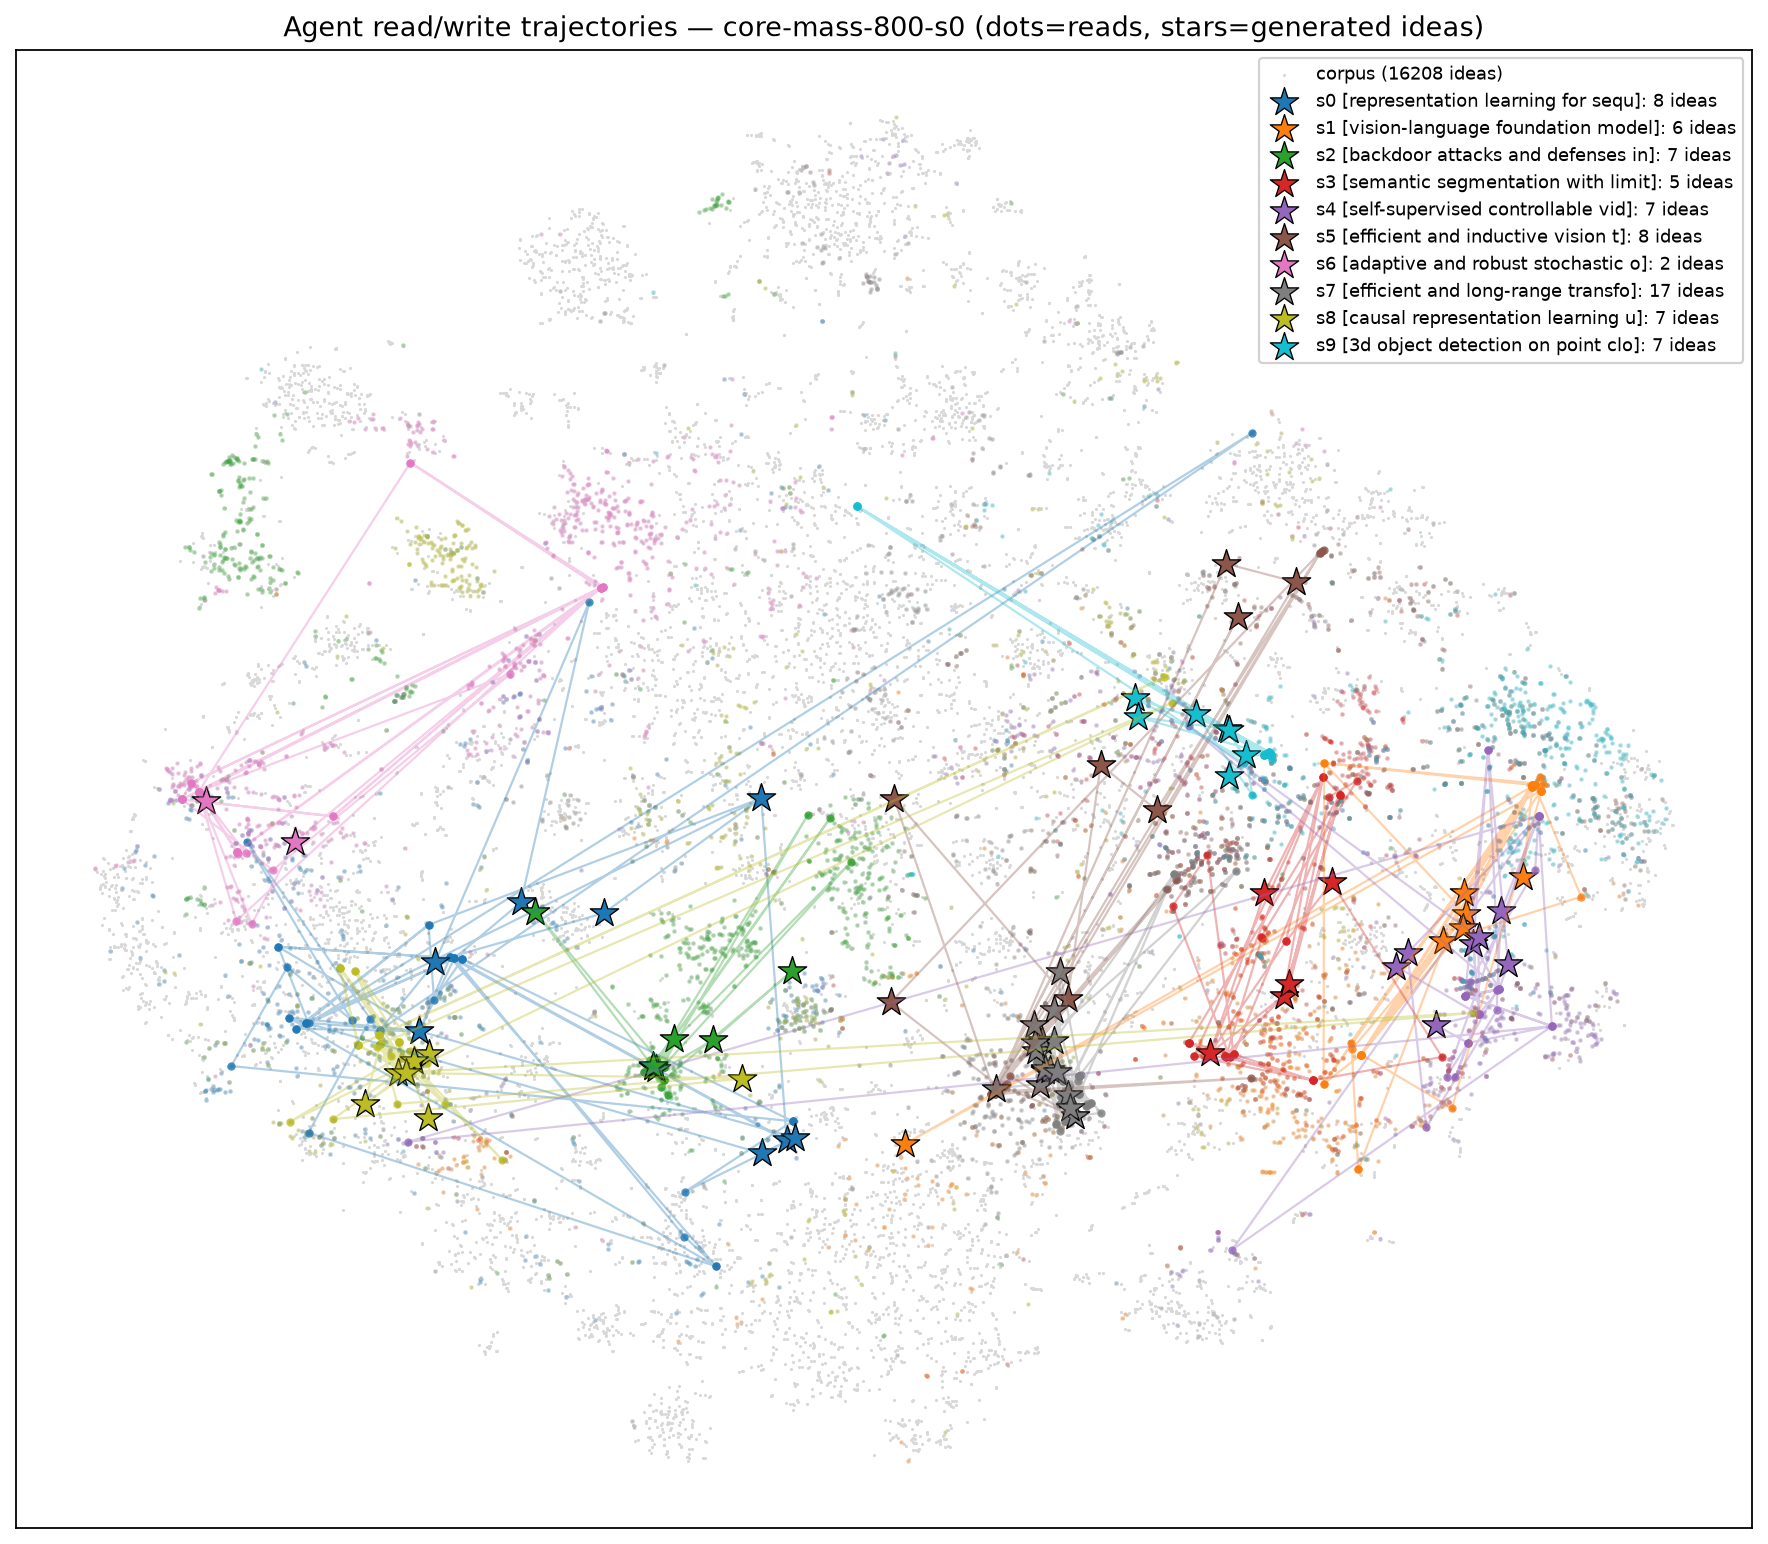
\includegraphics[width=\linewidth]{trajectories-c3.png}
\end{center}
\caption{Read/write trajectories of the ten specialists in the
$m{=}800$ condition on the fixed t-SNE map of the corpus. Tinted areas
are each agent's readable region; dots are reads, stars are generated
ideas. Although writing is unconstrained, specialists write inside or
near the regions they read.}
\label{fig:traj}
\end{figure}

\subsection{Agent action interface}
\label{app:actions}

Each agent interacts with the environment exclusively through the
following six actions, chosen one per turn by emitting a single JSON
object (\texttt{\{"action": ..., "args": \{...\}\}}); malformed replies
fall back to \texttt{sample\_frontier}. Every action returns a JSON
result---including scope-restriction errors, which the agent is
instructed to adapt to rather than retry.

\begin{itemize}
\item \texttt{search(query, k{=}5)} --- embed the query and return the
  top-$k$ nearest ideas \emph{within the agent's readable scope}
  (over-fetch then filter), each as node id, 300-character preview, and
  similarity score. This is the agents' primary discovery channel.
\item \texttt{browse(node\_id)} --- return the node's full idea text
  plus up to 10 outgoing (cited) and 10 incoming (citing) neighbors,
  each with a 200-character preview; neighbors outside the readable
  scope are filtered out. On an edgeless graph
  (Sec.~\ref{sec:noedges}) this degenerates to reading the node alone.
\item \texttt{sample\_frontier()} --- jump to one node drawn uniformly
  at random from the agent's readable scope; the serendipity channel.
  Disabled in the jump ablation (\texttt{allow\_jump{=}false}), in
  which case it returns a restriction error.
\item \texttt{generate(text, cited\_ids)} --- add a new idea node (a
  3--4 sentence paragraph) citing the existing ideas it builds on.
  Citation admissibility follows the \emph{read} scope (citing means
  having read): out-of-scope citations are dropped with notice, and the
  generate proceeds with the rest. The new node and its edges join the
  shared graph immediately and permanently.
\item \texttt{add\_links(src\_id, dst\_ids)} --- record missing
  reference links from an existing idea to ideas it builds on
  (curation).
\item \texttt{remove\_links(src\_id, dst\_ids)} --- remove reference
  links that do not actually support the source idea.
\end{itemize}

Each agent carries a FIFO memory of its last 20 (action, result) pairs,
rendered into every prompt together with a stable identity header (run
and agent id) and the action documentation; there is no other
communication channel between agents. Visible output is capped at
2{,}000 tokens per turn (reasoning tokens budgeted separately).

\subsection{Judge rubric}
\label{app:rubric}
Level 0: different problem entirely. 1: same broad area, different
goal. 2: same specific problem, unrelated approach. 3: same problem,
approaches in the same method family. 4: same problem and core
mechanism, differing in secondary components. 5: essentially the same
idea (problem, mechanism, and key design choices).

\subsection{Case studies: anticipations and their realizations}
\label{app:cases}

\textbf{Case 1 (realization level 5).} Agent g11 of the $N{=}50$
scaling run proposed:
\begin{quote}\small\itshape
We propose Conformal Early-Stopping Self-Consistency (CESS), a
black-box, distribution-free procedure that turns self-consistency
sampling into a risk-controlled stopping rule with finite-sample
guarantees. On a calibration set, we run deep self-consistency to learn
a mapping from the trajectory of vote-share (and simple diversity
features) to correctness, then derive nondecreasing stopping boundaries
via conformal calibration so that when the live vote-trajectory crosses
the boundary we stop and output the modal answer with $1-\alpha$
coverage; if the boundary is not reached within a budget, we abstain.
[\ldots]
\end{quote}
The judge matched it at level 5 to \emph{Black-Box Reliability
Certification for AI Agents via Self-Consistency Sampling and Conformal
Calibration} (arXiv, February 2026), with the evidence: ``the paper
implements black-box self-consistency sampling combined with conformal
calibration to produce sequential early-stopping rules with
finite-sample guarantees.''

\textbf{Case 2 (tier 1, level 4).} Agent g37 of the same run proposed
\emph{Path-of-Thought Distillation for text-rich graphs}: prompt an LLM
with ordered node/edge texts along candidate evidence paths to generate
structured relational rationales, then distill those rationales into a
hybrid tokenized graph transformer with attention-alignment and
counterfactual edge-text robustness losses, so that test-time inference
requires no LLM. The judge matched it at level 4 to \emph{Mitigating
Adversarial Attacks by Transferring LLM-generated Narrative Reasoning
for Robust Fake News Detection} (SIGIR 2026, a tier-1 venue): both
distill LLM-generated reasoning into graph models for robust graph
tasks with no runtime LLM, differing in the target domain.

\subsection{The 50-topic pool}
\label{app:topiclist}

{\small adaptive and robust stochastic optimization methods; efficient and inductive vision transformers; inductive and contextual knowledge graph representation; 3d object detection on point clouds; graph structure learning and generalization; evaluation and augmentation of language models; single-image to 3d generative modeling; continual learning and lifelong adaptation; causal representation learning under interventions; sparse neural network training and pruning; differentially private learning and optimization; self-supervised controllable video representation learning; task-oriented and knowledge-grounded dialogue modeling; efficient and long-range transformer architectures; adversarial robustness and training methods; offline and constrained reinforcement learning with pessimism; accelerated sampling and analysis of diffusion models; 3d generative models for molecular design; federated learning optimization and heterogeneity; learning-based combinatorial optimization methods; efficient model compression and adaptation for llms; semantic segmentation with limited supervision; foundation models and generative modeling for time series; multi-view graph-based clustering methods; language model alignment and calibration; efficient transfer and adaptation of models; backdoor attacks and defenses in ml models; out-of-distribution generalization and robustness; multi-step mathematical reasoning with lm prompts; evaluation and improvement of code generation models; retrieval-augmented multimodal question answering; contrastive representation learning and robustness; neural operator and physics-informed pde solvers; individual fairness and robustness in ML; representation learning for sequential decision making; multimodal representation learning for missing modalities; implicit bias and dynamics of deep learning; multimodal generative and robust audio models; language-models as autonomous decision agents; spatio-temporal traffic and trajectory modeling; vision-language foundation models and benchmarks; recommendation systems and sequential user modeling; offline reinforcement learning methods and theory; robust semi-supervised and noisy-label learning; interpretable and causally-grounded model explanations; few-shot and domain-adaptive object detection; high-resolution diffusion-based image synthesis; online learning and multiagent decision-making; out-of-distribution detection and outlier synthesis; embodied multimodal world-models for agents.}

\subsection{Recognized venues (tier 1)}
\label{app:venues}

Tier-1 recognition matches 60 venues by alias lists: the 58 venues rated A by the
CCF (2026 edition) across all categories, plus COLM and RLC. The full list:

{\small AAAI Conference on Artificial Intelligence; Neural Information Processing Systems; Annual Meeting of the Association for Computational Linguistics; Computer Vision and Pattern Recognition; IEEE International Conference on Computer Vision; International Conference on Machine Learning; International Conference on Learning Representations; Knowledge Discovery and Data Mining; International ACM SIGIR Conference on Research and Development in Information Retrieval; ACM SIGMOD International Conference on Management of Data; IEEE International Conference on Data Engineering; Very Large Data Bases; The Web Conference; ACM Multimedia; Conference on Language Modeling; Reinforcement Learning Conference; ACM SIGPLAN Symposium on Principles and Practice of Parallel Programming; USENIX Conference on File and Storage Technologies; Design Automation Conference; IEEE International Symposium on High Performance Computer Architecture; IEEE/ACM International Symposium on Microarchitecture; International Conference for High Performance Computing, Networking, Storage and Analysis; International Conference on Architectural Support for Programming Languages and Operating Systems; International Symposium on Computer Architecture; USENIX Annual Technical Conference; European Conference on Computer Systems; International Symposium on High-Performance Parallel and Distributed Computing; ACM SIGCOMM Conference; ACM International Conference on Mobile Computing and Networking; IEEE International Conference on Computer Communications; Symposium on Networked Systems Design and Implementation; ACM Conference on Computer and Communications Security; International Conference on the Theory and Applications of Cryptographic Techniques; IEEE Symposium on Security and Privacy; International Cryptology Conference; USENIX Security Symposium; Network and Distributed System Security Symposium; ACM SIGPLAN Conference on Programming Language Design and Implementation; ACM SIGPLAN-SIGACT Symposium on Principles of Programming Languages; ACM International Conference on the Foundations of Software Engineering; ACM Symposium on Operating Systems Principles; Conference on Object-Oriented Programming Systems, Languages, and Applications; International Conference on Automated Software Engineering; International Conference on Software Engineering; International Symposium on Software Testing and Analysis; USENIX Symposium on Operating Systems Design and Implementation; International Symposium on Formal Methods; ACM Symposium on the Theory of Computing; ACM-SIAM Symposium on Discrete Algorithms; International Conference on Computer Aided Verification; IEEE Annual Symposium on Foundations of Computer Science; ACM/IEEE Symposium on Logic in Computer Science; ACM SIGGRAPH; IEEE Conference on Virtual Reality and 3D User Interfaces; IEEE Visualization Conference; ACM Conference on Computer Supported Cooperative Work and Social Computing; ACM Conference on Human Factors in Computing Systems; ACM International Joint Conference on Pervasive and Ubiquitous Computing; ACM Symposium on User Interface Software and Technology; IEEE Real-Time Systems Symposium.}

Tier-2 additionally matches the $\sim$90 CCF-B venue aliases; the exact alias
lists (including abbreviation variants used for matching) ship with the released
configurations.

\subsection{Compute and cost}
\label{app:cost}

All experiments ran on commodity hardware; the only significant cost is
LLM API usage. Approximate totals: corpus distillation (16{,}208
summaries, \texttt{gpt-5-mini}) $\sim$\$15; the six dial runs (4{,}800
\texttt{gpt-5} actions) $\sim$\$90--150; the scaling runs (9{,}300
actions) $\sim$\$170--280; ablations (1{,}600 actions) $\sim$\$30--60;
evaluation (judging $\sim$1{,}000 ideas with \texttt{gpt-5-mini},
searches free) $\sim$\$40--80. Total on the order of \$350--600. A
single dial-style run (10 agents, 80 rounds) costs $\sim$\$15--25 and
$\sim$1 hour wall clock; evaluation of its ideas a further
$\sim$\$5--10.

\subsection{Behavioral observations}

\textbf{Onset.} Median personal round of an agent's first
\texttt{generate} action: 21--24 across conditions (minimum 9); the
first 40 rounds of a team are dominated by
\texttt{search}/\texttt{browse}. This is why the scaling experiment
fixes per-agent depth at 30 rounds: shallower budgets produce
(near-)zero output for any team size.

\textbf{Error-driven adaptation, and its memory horizon.} Constraints
are never described in the prompt; agents discover them through error
results. The jump ablation shows this cleanly: at cold start, 9 of 10
agents' very first action was \texttt{sample\_frontier} (their standard
opening move), each received the restriction error, and all switched to
\texttt{search}-based cold starts immediately. Across the remaining 790
actions only three further jump attempts occurred (team steps 400, 455,
719)---each long after the original error had been evicted from the
agent's 20-entry FIFO memory. The rolling memory length thus sets the
time scale on which learned constraints are forgotten.

\section{LLM usage}
\label{app:llm}

LLMs play three distinct roles in this work, disclosed here per the
ICLR 2026 LLM policy.

\textbf{As the object of study.} The agents whose dynamics we measure
are LLMs (\texttt{gpt-5}), and the evaluation judge, corpus distiller,
and topic namer are LLMs (\texttt{gpt-5-mini}). Every ``idea'' analyzed
in this paper is, by design, LLM-generated; all quantitative claims are
about LLM behavior.

\textbf{As research infrastructure.} The experimental platform ---
simulation environment, evaluation pipeline, and analysis code --- was
implemented with the assistance of an LLM-based coding agent operating
under continuous human direction. The human authors specified the
research questions, experimental designs, evaluation criteria, and all
design decisions (including mid-course redesigns reported in the
paper); the coding agent implemented, executed, and monitored the
experiments and proposed analyses that the authors accepted, rejected,
or redirected.

\textbf{In writing.} The manuscript was drafted with LLM assistance
from the authors' experimental records and instructions; the authors
reviewed and edited the text and take full responsibility for its
content. LLMs are not authors of this paper.

\end{document}
